\documentclass[12pt]{article}
\usepackage[a4paper]{geometry}
\usepackage[myheadings]{fullpage}
\usepackage{fancyhdr}
\usepackage{lastpage}
\usepackage{graphicx, wrapfig, subcaption, setspace, booktabs}
\usepackage{amsfonts,dcolumn}
\usepackage[T1]{fontenc}
\usepackage[font=small, labelfont=bf]{caption}
\usepackage{fourier}
\usepackage[protrusion=true, expansion=true]{microtype}
\usepackage[english]{babel}
\usepackage{sectsty}
\usepackage{url, lipsum}
\usepackage{listings}
\usepackage{float}

\lstdefinestyle{customc}{
  belowcaptionskip=1\baselineskip,
  breaklines=true,
  frame=L,
  xleftmargin=\parindent,
  language=Python,
  showstringspaces=false,
  basicstyle=\footnotesize\ttfamily,
  keywordstyle=\bfseries\color{green!40!black},
  commentstyle=\itshape\color{purple!40!black},
  identifierstyle=\color{blue},
  stringstyle=\color{orange},
}


\newcommand{\HRule}[1]{\rule{\linewidth}{#1}}
\onehalfspacing
\setcounter{tocdepth}{5}
\setcounter{secnumdepth}{5}

%-------------------------------------------------------------------------------
% HEADER & FOOTER
%-------------------------------------------------------------------------------
\pagestyle{fancy}
\fancyhf{}
\setlength\headheight{15pt}
\fancyhead[L]{Introduction to Computational and Data Science}
\fancyhead[R]{Stony Brook University}
\fancyfoot[R]{Page \thepage\ of \pageref{LastPage}}
%-------------------------------------------------------------------------------
% TITLE PAGE
%-------------------------------------------------------------------------------

\begin{document}
\begin{sloppypar}
\title{ \LARGE \textsc{AMS561 Final Project}
		\\ [2.0cm]
		\HRule{0.5pt} \\
		\LARGE \textbf{\uppercase{Graduate Admission Analysis}}
		\HRule{2pt} \\ [0.5cm]
		\normalsize \today \vspace*{5\baselineskip}}

\date{}


\author{\begin{tabular}{rl}
  \textbf{Name:} &Yifan Zhai\\
  \textbf{SBID:}  &112360276\\
  \textbf{Department:} & Technolog \& Society\\
  \textbf{Professor:} & Robert Harrison
\end{tabular}}

\maketitle
\thispagestyle{empty}
\newpage
\setcounter{page}{1}
\tableofcontents
\newpage


\section{Introduction}

\subsection{Data Resource}
This project uses a Graduate Admission [1] dataset which is inspired by the UCLA Graduate Dataset in an Indian perspective. The dataset is public and available on \texttt{kaggle}. \\
The size of the dataset has 400 entries and 9 variables with no NULL value. The first variable is the serial number of each student, which is not correlated with the chance of admission and I set it as the index of dataset. Other variables are  considered important during the application for Masters Programs, including : 1. GRE Scores ( out of 340 ) 2. TOEFL Scores ( out of 120 ) 3. University Rating ( out of 5 ) 4. Statement of Purpose (out of 5) 5. Letter of Recommendation Strength ( out of 5 ) 6. Undergraduate GPA ( out of 10 ) 7. Research Experience ( either 0 or 1 ) 8. Chance of Admit ( ranging from 0 to 1). Figure 1 below shows first few rows of the dataset to give you a initial cognition of the dataset.
\begin{figure}[H]
    \centering
    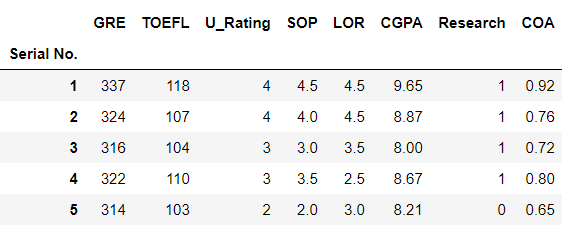
\includegraphics{head.png}
    \caption{First five rows of the dataset}
\end{figure}


\subsection{objective}

To apply for a master's degree is a very expensive and intensive work. There are many motley intermediary agents charges a lot to assist students applying for the graduate school. This project aims to generate a fair and sound analysis report to find the most relevant factors and their relationship with the chance of admission. Besides, students could use my models to guess their capacities and choose the most fitting graduate schools.\\
There are three outcomes for this project. Firstly, the distribution of students' test scores and other variables. Secondly, the most influential components. Lastly, the prediction of the probability that a student can be admitted to the college. Other details will be presented in the following sections. 

\section{Methods}

In this section, the techniques and tools used in the project will be covered in detail. 

\subsection{Language \& Environment}

This project is built in Jupiter Notebook in \texttt{Python 3}. Jupiter Notebook is an open-source web application supporting live code and clean text. Python 3 is an object-oriented high-level programming language released in 2008 [2]. I apply data cleaning, transformation, statistical modeling, data visualization and machine learning techniques to the dataset.
\subsection{Packages \& Tools}

Packages we imported includes: Numpy, Pandas, Matplot, Seaborn and scikit-learn.\\
Numpy is a fundamental package for scientific computing, I use its "array" tool in this project. Pandas, derived from "panel data", is a software library written for the Python programming language for data manipulation and analysis [3]. This project use pandas to load and manipulate the dataset. Seaborn is a Python data visualization library based on matplotlib [5], it has many strong tools including \texttt{boxplot}, \texttt{heatmap} and \texttt{pairplot}\\
Scikit-learn, short for sklearn, is a machine learning package in Python with many efficient tools for data mining. It is built on NumPy, SciPy and matplotlib [4]. The tools used in our project incudes: 
\begin{enumerate}
    \item model\_selection: dividing the dataset into training set and test set.
    \item linear\_model: building linear model and predict on the test dataset.
    \item metrics: building confusion matrix, calculating precision score, recall score, accuracy score and $r^2$ score. 
    \item trees: including decision tree regression model and decision tree classification model
    \item ensemble: including random foreset regression model and random forest classification model
    \item neighbors: building k nearest neighbors model, which is supervised learning
    \item svm: support vector machine, a classification model
\end{enumerate}

\section{Results}

\subsection{Correlation Between Columns}

Firstly, I use the \texttt{heatmap} (Figure 2) to visualize the correlation between every two columns so that we can get a primary cognition of the relationship in the dataset.

\begin{figure}[H]
    \centering
    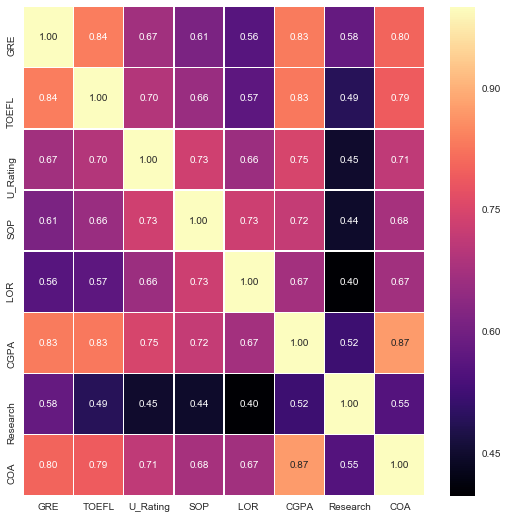
\includegraphics[scale = 0.8]{corr_heatmap.png}
    \caption{Correlation Heatmap }
\end{figure}
In the heatmap, it is obvious that 3 most important features for admission to the Master are CGPA ("College GPA"), GRE SCORE and TOEFL SCORE. Therefore, we want to go for more details about the relationship between these three variables and chance of admission. The pair plot (Figure 3) with the students having research experience or not is presented.

\begin{figure}[H]
    \centering
    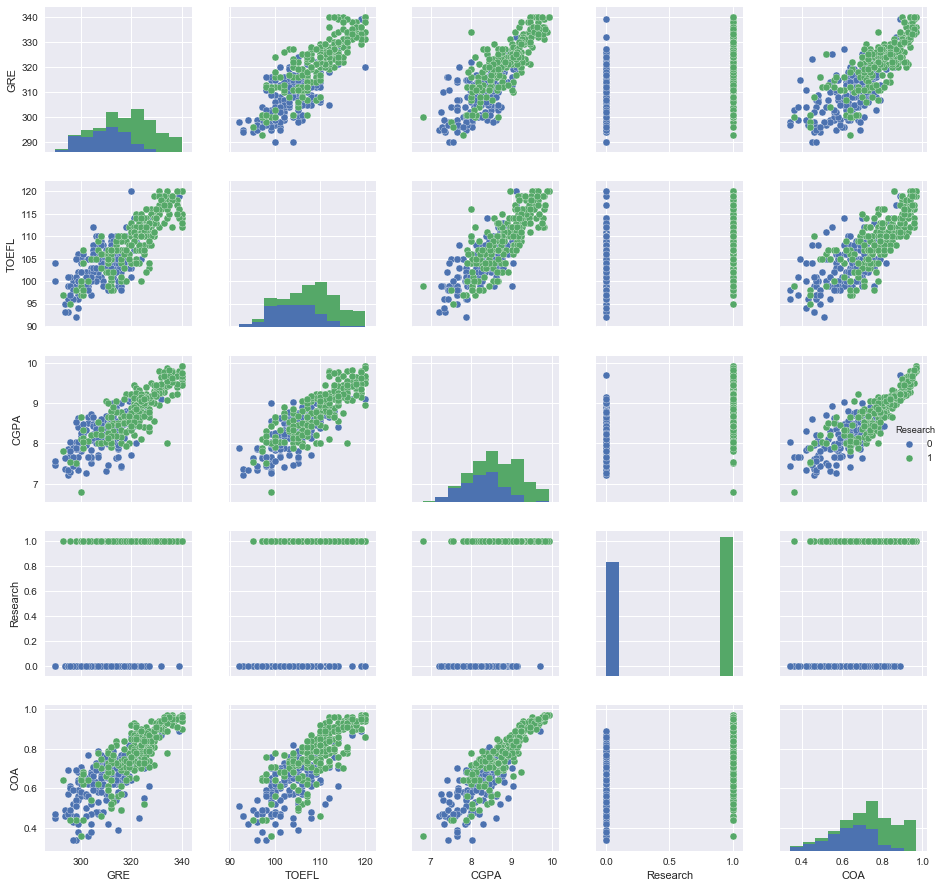
\includegraphics[scale = 0.46]{pair_plot.png}
    \caption{Pair Plot}
\end{figure}

From the pair plot, GRE, TOEFL and CGPA appears to be positive linear related to the Chance of Admission. Therefore, we should consider using linear regression model afterwards. Besides, students with research experience tend to have higher GRE, TOEFL Score, CGPA and higher Chance of Admission eventually. Before building models, let's take a look into the distribution of these three important variables and Chance of Admission.\\


\begin{figure}[H]
    \centering
    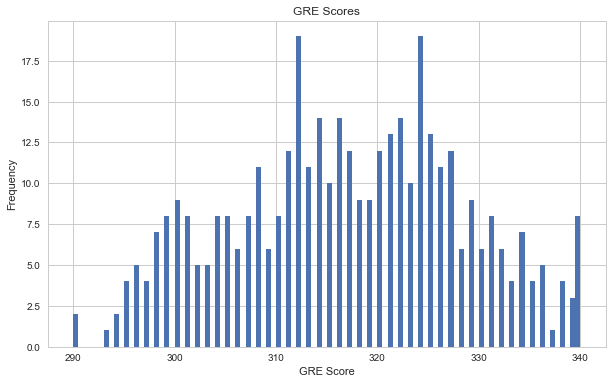
\includegraphics[scale = 0.6]{GRE.png}
    \caption{GRE Distritbution}
\end{figure}
 
 \begin{figure}[H]
 \centering
  \begin{subfigure}[b]{0.45\textwidth}
    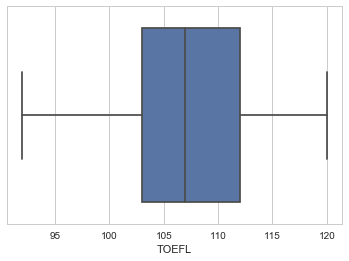
\includegraphics[width=\textwidth]{TOEFL.png}
    \caption{TOEFL Distribution}
    \label{fig:1}
  \end{subfigure}
  %
  \begin{subfigure}[b]{0.45\textwidth}
    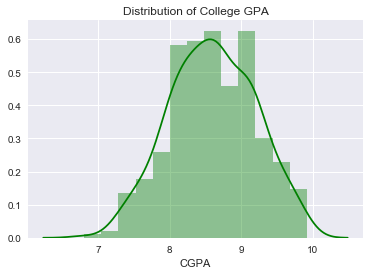
\includegraphics[width=\textwidth]{CGPA.png}
    \caption{CGPA Distribution}
    \label{fig:2}
  \end{subfigure}
\end{figure}
 





\begin{figure}[H]
    \centering
    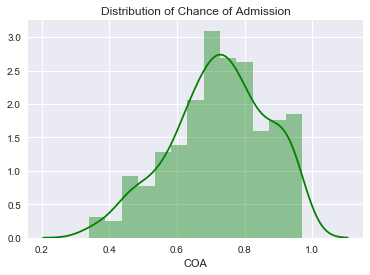
\includegraphics[scale = 1]{COA.png}
    \caption{Pair Plot}
\end{figure}

\section{Reference}

\begin{enumerate}
    \item Mohan S Acharya, Asfia Armaan, Aneeta S Antony : A Comparison of Regression Models for Prediction of Graduate Admissions, IEEE International Conference on Computational Intelligence in Data Science 2019
    \item \url{https://www.tutorialspoint.com/python3/}
    \item \url{https://en.wikipedia.org/wiki/Pandas_(software)}
    \item \url{https://scikit-learn.org/stable/}
    \item \url{https://seaborn.pydata.org/}
\end{enumerate}



\end{sloppypar}
\end{document}